\documentclass[11pt,oneside]{article}
\input{../../../Header/packages.sty}
\input{../../../Header/styleScript.sty}
\input{../../../Header/headerScript.sty}
\input{../../../Header/mathexpressions.sty}


\newcommand{\Skriptname}{Lektion: Der Höhensatz}
\newcommand{\Autor}{Jonas Guler (Gu)}
\newcommand{\version}{\textit{v}1.0}

\begin{document}
\thispagestyle{plain}
\begin{center}
	{\Huge\textbf{Der Höhensatz}}\\[3mm]
	{\large Sätze im rechtwinkligen Dreieck -- Aufbau auf Pythagoras und Kathetensatz}\\[2mm]
	{\normalsize Name: \gap{6}\hspace{1cm} Datum: \gap{3}}
\end{center}
\vspace{2mm}
Wir verwenden wieder die Bezeichnungen aus dem Skript: Im rechtwinkligen Dreieck $\triangle ABC$ mit $\gamma=90^\circ$ ist $c$ die Hypotenuse, $a$ und $b$ sind die Katheten. Die Höhe $h_c$ teilt die Hypotenuse in die Hypotenusenabschnitte $p$ (bei $A$, also an der Kathete $b$) und $q$ (bei $B$, also an der Kathete $a$). Aus der letzten Lektion kennen wir den Kathetensatz $a^2=c\cdot q$ und $b^2=c\cdot p$.
\begin{center}
	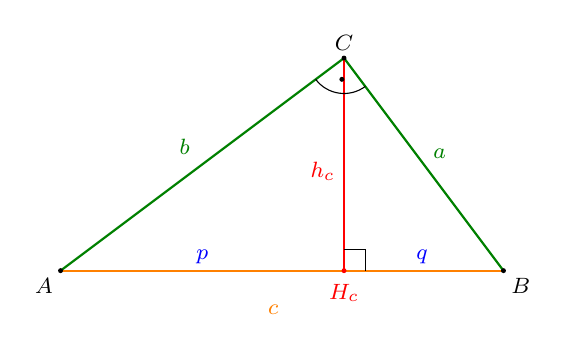
\begin{tikzpicture}[x=1cm, y=1cm, >=latex, font=\footnotesize, scale=0.9]
		\coordinate (A) at (0,0);
		\coordinate (B) at (6.25,0);
		\coordinate (C) at (4,3);
		\coordinate (H) at (4,0);
		\draw[color=orange, line width=0.8pt] (A) -- (B);
		\draw[color=green!50!black, line width=0.8pt] (B) -- (C) -- (A);
		\draw[color=red, line width=0.8pt] (C) -- (H);
		% rechte Winkel
		\draw [shift={(4,3)}] (-143.13:0.5) arc (-143.13:-53.13:0.5);
		\fill (3.97,2.7) circle (1pt);
		\draw (4.3,0) -- (4.3,0.3) -- (4,0.3);
		\begin{scriptsize}
			\fill (A) circle (1pt) node[below left] {$A$};
			\fill (B) circle (1pt) node[below right] {$B$};
			\fill (C) circle (1pt) node[above] {$C$};
			\fill[red] (H) circle (1pt) node[below=2pt, red] {$H_c$};
			\draw[color=orange] (3,-0.55) node {$c$};
			\draw[color=green!50!black] (5.35,1.65) node {$a$};
			\draw[color=green!50!black] (1.75,1.75) node {$b$};
			\draw[color=red] (3.7,1.4) node {$h_c$};
			\draw[color=blue] (2,0.2) node {$p$};
			\draw[color=blue] (5.1,0.2) node {$q$};
		\end{scriptsize}
	\end{tikzpicture}
\end{center}

%############################################################################################
\section{Einstieg: Höhe und Hypotenusenabschnitte}
\begin{aufgabe}[Entdeckungsaufgabe, Partnerarbeit] % Idee: Geometrie 1 Aufgaben (Niederberger) Kap. 5.2 Nr. 40
	\textbf{Teil A: Konstruieren und vermuten.} Beim Kathetensatz haben wir die Katheten mit den Hypotenusenabschnitten verglichen. Jetzt untersuchen wir, wie die Höhe $h_c$ mit $p$ und $q$ zusammenhängt.
	\begin{enumerate}[label=\alph*)]
		\item Konstruiere das rechtwinklige Dreieck $\triangle ABC$ mit $\gamma=90^\circ$ aus $p=4.5$ cm und $q=2$ cm. \textit{Tipp: Zeichne zuerst die Hypotenuse mit dem Punkt $H_c$. Wo muss $C$ liegen, damit bei $C$ ein rechter Winkel entsteht?}
		\item Miss die Höhe $h_c$ möglichst genau.
	\end{enumerate}
	\karos{6}
	\begin{enumerate}[label=\alph*), resume]
		\item Übertrage deinen Messwert in die Tabelle und ergänze die fehlenden Werte. Die Höhen der anderen Dreiecke sind bereits berechnet.
	\end{enumerate}
	\begin{center}
		\renewcommand{\arraystretch}{1.8}
		\begin{tabular}{|*{6}{>{\centering\arraybackslash}p{13mm}|}}\hline
			$p$ & $q$ & $c=p+q$ & $h_c$ & $h_c^2$ & $p\cdot q$ \\\hline\hline
			$4.5$ & $2$ & & & & \\\hline
			$8$ & $2$ & & $4$ & & \\\hline
			$2.5$ & $10$ & & $5$ & & \\\hline
			$1$ & $9$ & & $3$ & & \\\hline
		\end{tabular}
	\end{center}
	\begin{enumerate}[label=\alph*), resume]
		\item Was fällt dir auf? Formuliere eine Vermutung in Worten und als Formel.
	\end{enumerate}
	\karos{2.5}\\[3mm]
	\textbf{Teil B (für Schnelle): Ein Beweis nur mit Pythagoras.} Betrachte ein allgemeines rechtwinkliges Dreieck wie in der Figur oben.
	\begin{enumerate}[label=\alph*), resume]
		\item Drücke $a^2$ und $b^2$ mit Hilfe der Teildreiecke durch $h_c$, $p$ und $q$ aus.
		\item Setze deine beiden Terme in $a^2+b^2=c^2=(p+q)^2$ ein und vereinfache so weit wie möglich. Was erhältst du?
	\end{enumerate}
	\karos{5}
\end{aufgabe}

\newpage
%############################################################################################
\section{Der Höhensatz}
Auch diese Vermutung gilt in jedem rechtwinkligen Dreieck. Wie beim Kathetensatz vergleicht sie die Fläche eines Quadrates mit der Fläche eines Rechtecks.
\begin{satz}[Höhensatz]
	\begin{minipage}{0.5\linewidth}
		In einem rechtwinkligen Dreieck ist das Quadrat über der Höhe zur Hypotenuse flächengleich wie das Rechteck aus den \textbf{beiden Hypotenusenabschnitten}:
		\[h_c^2=p\cdot q.\]
	\end{minipage}
	\hfill
	\begin{minipage}{0.45\linewidth}
		\centering
		\begin{tikzpicture}[x=1cm, y=1cm, >=latex, font=\footnotesize, scale=0.62]
			% Dreieck: A(0,0), B(5,0), C(3.2,2.4); p=3.2, q=1.8, h=2.4
			\filldraw[fill=myblue, fill opacity=0.25, draw=black] (0.8,0) -- (3.2,0) -- (3.2,2.4) -- (0.8,2.4) -- cycle;
			\filldraw[fill=orange, fill opacity=0.25, draw=black] (0,0) -- (3.2,0) -- (3.2,-1.8) -- (0,-1.8) -- cycle;
			\draw[line width=1pt] (0,0) -- (5,0) -- (3.2,2.4) -- cycle;
			\draw[red, line width=1pt] (3.2,2.4) -- (3.2,0);
			\draw[dashed, ->] (5,0) arc (0:-90:1.8);
			\begin{scriptsize}
				\draw (-0.1,-0.1) node[left] {$A$};
				\draw (5.1,-0.1) node[right] {$B$};
				\draw (3.2,2.5) node[above] {$C$};
				\draw (1.7,1.5) node {$h_c^2$};
				\draw (1.6,-0.9) node {$p\cdot q$};
				\draw (1.6,-2.1) node {$p$};
				\draw (3.5,-0.9) node {$q$};
				\draw (4.1,0.25) node {$q$};
				\draw[red] (3.5,1.3) node {$h_c$};
			\end{scriptsize}
		\end{tikzpicture}
	\end{minipage}
\end{satz}
\begin{beweis}
	Wir benutzen den Satz des Pythagoras im Teildreieck $\triangle AH_cC$ und den Kathetensatz:
	\[\text{(I)}\ h_c^2=\gap{2.5} \qquad\text{(Pythagoras)}, \qquad\qquad \text{(II)}\ b^2=\gap{2} \qquad\text{(Kathetensatz)}\]
	\karos{2.5}
\end{beweis}
\textbf{Bemerkungen:}
\begin{itemize}
	\item Aus dem Höhensatz folgt $h_c=\sqrt{p\cdot q}$. Man nennt $\sqrt{p\cdot q}$ das \textbf{geometrische Mittel} der Zahlen $p$ und $q$.\\ Die Höhe ist also das geometrische Mittel der beiden Hypotenusenabschnitte.
	\item Im Höhensatz spielt es keine Rolle, welcher Abschnitt $p$ und welcher $q$ heisst. \textbf{Achtung:} Es muss aber die Höhe \textbf{auf die Hypotenuse} sein. Merke dir den Satz in Worten: \textit{Höhe$^2$ = Produkt der beiden Hypotenusenabschnitte}.
	\item Damit haben wir die ganze \textbf{Satzgruppe des Pythagoras} beisammen:
	\begin{center}
		\renewcommand{\arraystretch}{1.6}
		\begin{tabular}{|l|p{45mm}|p{55mm}|}\hline
			\textbf{Satz} & \textbf{Formel} & \textbf{in Worten}\\\hline
			Pythagoras & & \\\hline
			Kathetensatz & & \\\hline
			Höhensatz & & \\\hline
		\end{tabular}
	\end{center}
\end{itemize}

\begin{beispiel}
	Im rechtwinkligen Dreieck $\triangle ABC$ mit $\gamma=90^\circ$ sind $q=4$ cm und $h_c=6$ cm gegeben. Berechne $p$, $c$, die Katheten $a$ und $b$ sowie den Flächeninhalt des Dreiecks. Kontrolliere den Flächeninhalt mit $\frac{a\cdot b}{2}$.
\end{beispiel}
\karos{5}

%############################################################################################
\section{Übungen}
\setcounter{aufg}{0}
\begin{aufgabe}[Grundaufgaben] % angelehnt an Geometrie 1 Aufgaben Kap. 5.2 Nr. 43 und Geometrie 2 (Niederberger) S. 84 Nr. 2, 6
	Berechne in den rechtwinkligen Dreiecken $\triangle ABC$ mit $\gamma=90^\circ$ (Bezeichnungen wie in der Figur auf Seite 1) die gesuchten Grössen. Mache jeweils eine Skizze.
	\begin{enumcols}[2]
		\item $p=8$ cm, $q=2$ cm. Gesucht: $h_c,a,b$.
		\item $h_c=12$ cm, $p=16$ cm. Gesucht: $q,c$.
		\item $h_c=6$ cm, $q=3$ cm. Gesucht: $p,a,b$.
		\item $c=10$ cm, $p=2$ cm. Gesucht: $q,h_c,b$.
		\item $b=5$ cm, $p=3$ cm. Gesucht: $h_c,q,c$.
		\item $a=13$ cm, $h_c=12$ cm. Gesucht: $q,p,c$.
	\end{enumcols}
	\karos{11}
\end{aufgabe}

\begin{aufgabe}[Abschnitte im Verhältnis]
	In einem rechtwinkligen Dreieck mit $\gamma=90^\circ$ misst die Hypotenuse $c=15$ cm. Der Hypotenusenabschnitt $p$ ist viermal so lang wie $q$. Berechne $p$, $q$, $h_c$ und den Flächeninhalt des Dreiecks.\par
	\karos{5}
\end{aufgabe}

\begin{aufgabe}[Ein Rechteck wird zum Quadrat] % angelehnt an Geometrie 2 (Niederberger) S. 84 Nr. 1 und Geometrie 1 Aufgaben Nr. 41a
	Mit dem Höhensatz lässt sich ein Rechteck in ein flächengleiches Quadrat verwandeln. Gegeben ist ein Rechteck mit den Seitenlängen $6$ cm und $2$ cm.
	\begin{enumerate}[label=\alph*)]
		\item Zeichne eine Strecke $\overline{AB}$ der Länge $6+2=8$ cm und markiere darauf den Punkt $H$ mit $\overline{AH}=6$ cm.
		\item Errichte in $H$ die Senkrechte zu $AB$ und zeichne den Thaleskreis über $\overline{AB}$. Der Schnittpunkt der beiden ist $C$.
		\item Begründe mit dem Höhensatz, weshalb das Quadrat über $\overline{HC}$ denselben Flächeninhalt hat wie das Rechteck. Zeichne das Quadrat.
		\item Berechne $\overline{HC}$ und kontrolliere deine Zeichnung durch Messen.
		\item Vergleiche mit der Konstruktion über den Kathetensatz aus der letzten Lektion: Was ist gleich, was ist anders?
	\end{enumerate}
	\karos{9}
\end{aufgabe}

\begin{aufgabe}[Wurzeln konstruieren] % Idee: Geometrie 2 (Niederberger) S. 84 Nr. 5
	Konstruiere mit Hilfe des Höhensatzes eine Strecke der Länge
	\begin{enumcols}[2]
		\item $\sqrt{10}$ cm,
		\item $\sqrt{7}$ cm.
	\end{enumcols}
	Beschreibe kurz, wie du $p$ und $q$ gewählt hast. Gibt es mehrere Möglichkeiten?\par
	\karos{7}
\end{aufgabe}

\begin{aufgabe}[Der Tunnel]
	Ein Tunnel hat einen halbkreisförmigen Querschnitt mit einem Durchmesser von $10$ m.
	\begin{enumerate}[label=\alph*)]
		\item Wie hoch ist der Tunnel $1.5$ m vom Rand entfernt? \textit{Tipp: Thaleskreis.}
		\item Passt ein $2.5$ m breiter und $4.5$ m hoher Lastwagen durch den Tunnel, wenn er genau in der Mitte fährt?
		\item $\bigstar$ Wie breit darf ein $4$ m hoher Lastwagen höchstens sein, damit er in der Mitte gerade noch durch den Tunnel passt?
	\end{enumerate}
	\karos{7}
\end{aufgabe}

\begin{aufgabe}[$\bigstar$ Knobelaufgabe: Zwei Mittelwerte] % Idee: Geometrie 2 (Niederberger) S. 84, Aufgaben zur Vertiefung Nr. 1
	Für zwei positive Zahlen $p$ und $q$ heisst $\frac{p+q}{2}$ das \textbf{arithmetische Mittel} und $\sqrt{p\cdot q}$ das \textbf{geometrische Mittel}.
	\begin{enumerate}[label=\alph*)]
		\item Zeichne einen Halbkreis über einer Strecke der Länge $p+q$ (z.B. $p=7$ cm, $q=2$ cm) und finde in der Figur je eine Strecke, die so lang ist wie das arithmetische bzw.\ das geometrische Mittel.
		\item Begründe mit der Figur, weshalb immer $\sqrt{p\cdot q}\leq\frac{p+q}{2}$ gilt. Wann gilt das Gleichheitszeichen?
	\end{enumerate}
	\karos{6}
\end{aufgabe}

\end{document}
